\begin{figure*}[htbp]
    \centering
    \begin{tabular}{m{43mm} m{43mm} m{43mm} m{43mm} m{10mm}}
        \hspace{-3mm}
        \begin{minipage}[b]{\linewidth}
            \centering
            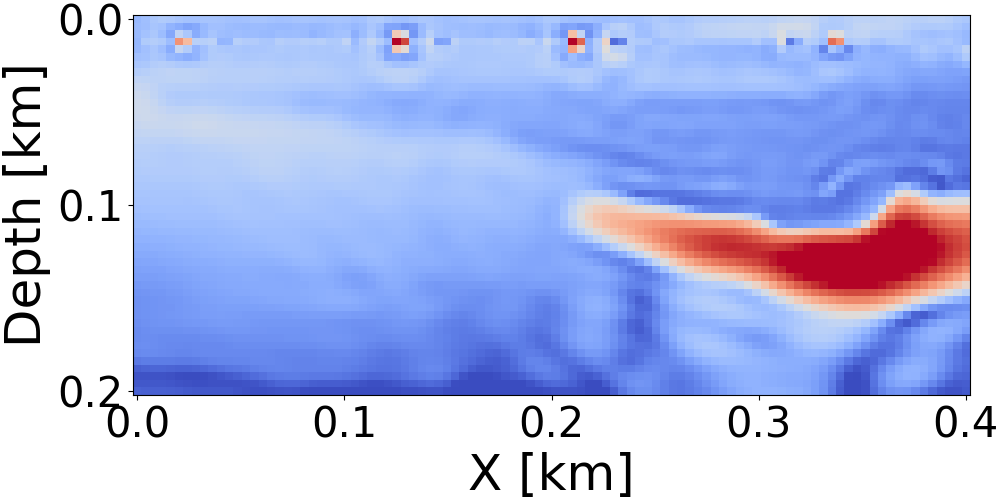
\includegraphics[width=\linewidth]{public/gradient}
%            \vspace{-6mm}
            \caption*{(a) Standard FWI}
%            \vspace{1mm}
        \end{minipage} &
        \hspace{-8mm}
        \begin{minipage}[b]{\linewidth}
            \centering
            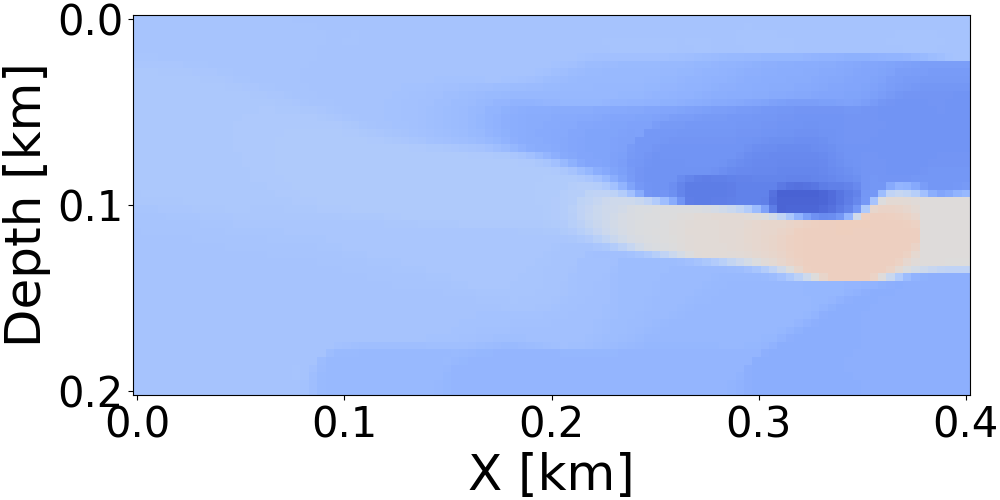
\includegraphics[width=\linewidth]{public/alpha_150}
%            \vspace{-6mm}
            \caption*{(b) Proposed, $\alpha$ = 150}
%            \vspace{1mm}
        \end{minipage} &
        \hspace{-13mm}
        \begin{minipage}[b]{\linewidth}
            \centering
            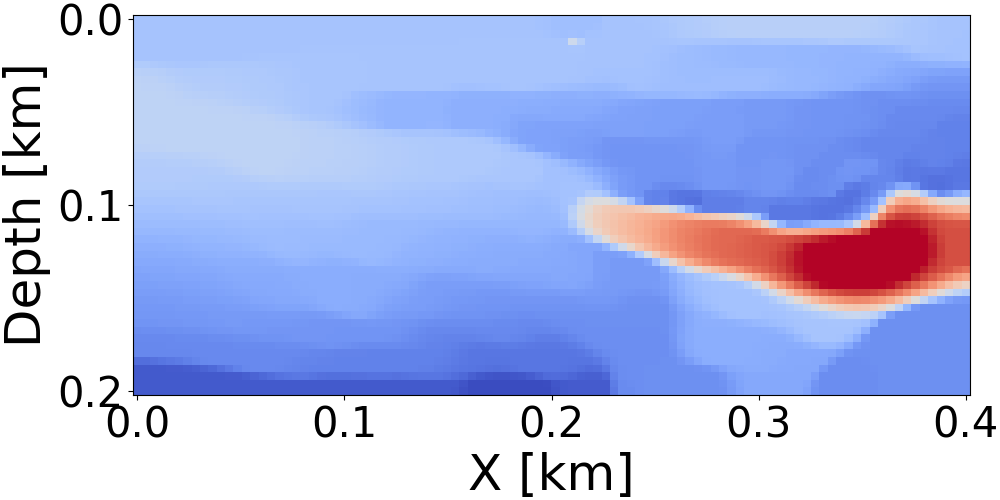
\includegraphics[width=\linewidth]{public/alpha_350}
%            \vspace{-6mm}
            \caption*{(c) Proposed, $\alpha$ = 350}
%            \vspace{1mm}
        \end{minipage} &
        \hspace{-18mm}
        \begin{minipage}[b]{\linewidth}
            \centering
            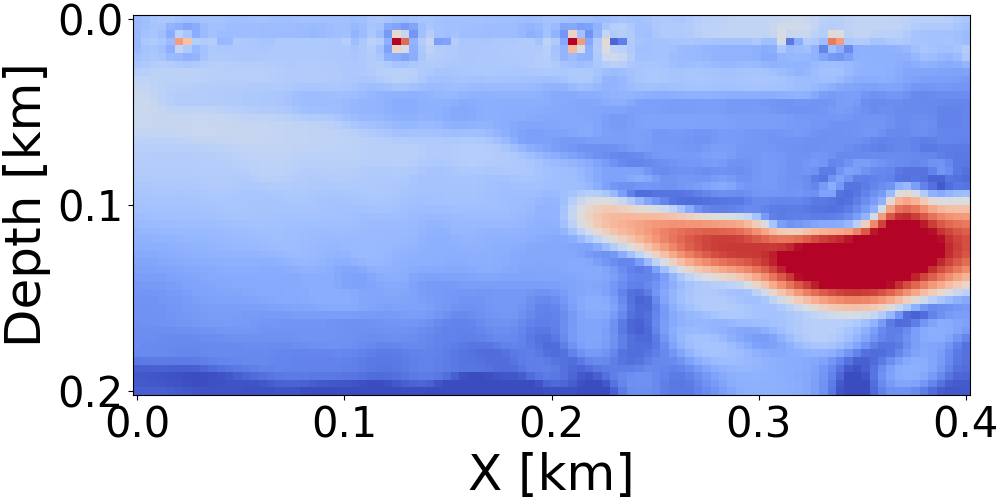
\includegraphics[width=\linewidth]{public/alpha_550}
%            \vspace{-6mm}
            \caption*{(d) Proposed, $\alpha$ = 550}
%            \vspace{1mm}
        \end{minipage} &
%        \hspace{-18mm}
%        \multirow[t]{3}{*}{\raisebox{-5mm}{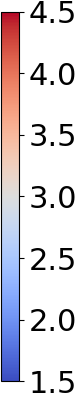
\includegraphics[height=20mm]{public/color-bar}}} \\
    \end{tabular}
%    \vspace{-3mm}
    \captionsetup{margin=1cm}
    \caption{
        Velocity models [km/s] and their corresponding reconstructions. (c) is the best reconstruction result. \\
        (b) is over-smoothed with a stronger TV constraint, and (d) similar results to (a) with a weaker one.
    }
%    \vspace{-4mm}
    \vspace{1mm}
    \label{fig:velocity-models-pure}
\end{figure*}
